\documentclass[12pt, letterpaper, twoside, openany, pdftex]{thesis}
%	\includeonly{./tex/introduction}
%	\includeonly{./tex/time_stability}
%	\includeonly{./tex/fiber_impairments}
%	\includeonly{./tex/results}
%	\includeonly{./tex/conclusion}

%	\includeonly{./tex/fiber_impairments, ./tex/results}
	
	%\usepackage[T1]{fontenc}
	%\usepackage[utf8]{inputenc}
	
	\usepackage{amsmath}
	\usepackage{amsfonts}
	\usepackage{amssymb}
	
	\usepackage{setspace}
	
	\usepackage{graphicx}
	\usepackage{tikz}
	\usepackage{cite}
	\usepackage{hhline}
	\usepackage{multirow}

	\usepackage{caption}
	\captionsetup{justification=raggedright,singlelinecheck=false}
	
	\usepackage{tabls}

	\usepackage{titlesec}
		\titleformat{\chapter}
		{\normalfont\large\bfseries}{Chapter \thechapter:}{1em}{}

		\titleformat{\section}
		{\normalfont\large\bfseries}{\thesection}{1em}{}
		
		\titleformat{\subsection}
		{\normalfont\large}{\thesubsection}{1em}{}

% Differentiation
\renewcommand*{\d}{\mathrm{d}}
\newcommand*{\dd}{\partial}

\newcommand*{\diffp}[2]{\ensuremath{\frac{\dd #1}{\dd #2}}}
\newcommand*{\difff}[2]{\ensuremath{\frac{\d #1}{\d #2}}}
\newcommand*{\diffff}[3]{\ensuremath{\frac{\d^2 #1}{\d #2 \d #3}}}
\newcommand*{\D}{\mathcal{D}}
\newcommand*{\I}{\mathcal{I}}
\def\ip #1#2{\lbrack\!\lbrack #1 | #2 \rbrack\!\rbrack}



	
%	\doublespacing
%	\setstretch{2}
%	\openup 1em



\newcommand{\tbsp}{\rule{0pt}{18pt}} %used to get a vertical distance after \hline
\renewcommand{\baselinestretch}{2}
\setlength{\textwidth}{5.9in}
\setlength{\textheight}{9in}
\setlength{\topmargin}{-.50in}
%\setlength{\topmargin}{0in}    %use this setting if the printer makes the the top margin 1/2 inch instead of 1 inch
\setlength{\oddsidemargin}{.55in}
\setlength{\parindent}{.4in}
\pagestyle{empty}


	
\begin{document}
	%Abstract Page 

\hbox{\ }

\renewcommand{\baselinestretch}{1}
\small \normalsize

\begin{center}
\large{{ABSTRACT}} 

\vspace{2em} 

\end{center}
\hspace{-.15in}
\begin{tabular}{ll}
Title of dissertation:    & {\large  NONLINEAR INTERACTION BETWEEN }\\
&				      {\large  A FREQUENCY SIGNAL AND NEIGHBORING} \\
&				      {\large  DATA CHANNELS IN A COMMERCIAL} \\
&				      {\large  OPTICAL FIBER COMMUNICATION SYSTEM} \\
\ \\
&                          {\large  Patrick Sykes, Master of Science, 2018} \\
\ \\
Dissertation directed by: & {\large  Dr. Curtis Menyuk, Professor} \\
&  				{\large	 Computer Science and Electrical Engineering} \\
\end{tabular}

\vspace{2em}

\renewcommand{\baselinestretch}{2}
\large \normalsize

We theoretically investigate the feasibility of transmitting a frequency signal in an interstice of the data channels in a commercial wavelength division multiplexed optical fiber communications system.  
We will give an overview of some different measures used for frequency stability. 
We also list the typical optical impairments that affect light propagating in an optical fiber and how the impairments can induce phase noise in a frequency signal.
The phase noise on the frequency signal due to the optical impairments can be limited by restricting the optical power, bandwidth, and center frequency of the signal.
The primary source of phase noise is cross-phase modulation (XPM) between the frequency signal and its neighboring data channels.
We calculate the first order structure functions and Allan deviation of the phase noise resulting from XPM as the averaging time varies using typical commercial system parameters. 
We find that the instability added by this effect is comparable to experimentally observed instabilities in research networks, suggesting that frequency transfer over commercial networks without occupying an entire data channel should be feasible.

	\thispagestyle{empty}
\hbox{\ }
\vspace{1in}
\renewcommand{\baselinestretch}{1}
\small\normalsize
\begin{center}

\large{{Nonlinear Interaction between  Neighboring Data Channels and a Frequency Signal in a Commercial Optical Fiber Communication System}}\\
\ \\
\ \\
\large{by} \\
\ \\
\large{Patrick Sykes}%Your full name as it appears in University records.
\ \\
\ \\
\ \\
\ \\
\normalsize
\end{center}

\vspace{7.5em}

	%Copyright

\thispagestyle{empty}
\hbox{\ }

\vfill
\renewcommand{\baselinestretch}{1}
\small\normalsize

\vspace{-.65in}

\begin{center}
\large{\copyright \hbox{ }Copyright by\\
Patrick Sykes  %Type your name as it appears in University records
\\
2018}
\end{center}

\vfill

	
	\pagestyle{plain}
	\pagenumbering{roman}
	\setcounter{page}{2}
	
	\renewcommand{\baselinestretch}{1}
	\small\normalsize
	
	\tableofcontents
	\newpage
	\listoffigures
	\listoftables
	\newpage
	
	\setlength{\parskip}{0em}
	\renewcommand{\baselinestretch}{2}
	\small\normalsize

	\pagenumbering{arabic}
	\setcounter{page}{1}
	\chapter{Introduction}

Improvements in optical frequency references allow them to be more precise than current atomic clock standards at microwave frequencies \cite{ProgressOpticalClock, RedefinitionOfSecond, Diddams2004}. It is expected that this greater precision will ultimately lead to a redefinition of the second, and greater precision and accuracy in timekeeping \cite{RedefinitionOfSecond}. It is desirable for many applications to transmit time and frequency from highly accurate and precise references, like those at the National Institute of Standards and Technology (NIST) or the US Naval Observatory (USNO), to distant locations. However, the transmission medium distorts the time and frequency data --- degrading their accuracy and precision.


%This opens up the potential to improve precision and accuracy in timekeeping systems as well as a redefinition of the second. That increase in precision and accuracy are limited by the synchronisation between those clocks using optical standards. There is some frequency uncertainty in a reference which becomes exacerbated as the reference is transmitted through a medium and influenced by the environment. Understanding the mechanisms for frequency distortion and controlling them where possible give stricter bounds on the frequency error.


Numerous systems require accurate timekeeping, including Global Positioning System (GPS) satellites and receivers, transaction logging, and certain research experiments \cite{ScienceOfTimekeeping}. Techniques and systems exist for time and frequency transfer in wireless communication systems.  A commonly-used method is two-way satellite time and frequency transfer, which makes it possible for two laboratories to use a satellite as a common link to synchronize their clocks. These wireless systems are typically accurate to within $1-10$ ns \cite{Allan1980}, which is sufficient for many applications, but far less accurate than the best primary references \cite{NISTFreqStandards, Audoin1976}. Additionally, satellites are physically inaccessible, which makes hardware maintenance and upgrades difficult and alse makes the satellites vulnerable to attack. Fiber optics are a potential substitute for land-based transfer, especially if one can take advantage of the existing fiber telecommunications infrastructure.


Research networks are increasingly transmitting time and frequency signals along with data over fiber optic communication systems. These networks include the R\'eseau Fibr\'e M\'etrologique \`a Vocation Europ\'eenne (REFIMEVE+) in France \cite{cantin2017progress}, PIONIER in Poland \cite{Turza2017}, 
and the White Rabbit networks used at the CERN accelerator sites and GSI's Facility for Antiproton and Ion Research \cite{Serrano2013}.  
A larger European optical time and frequency distribution network called CLONETS is planned \cite{CLONETS}.
The REFIMEVE+ project has demonstrated frequency transfer over optical fibers with a stability of $10^{-16}$ at $1$ s and $10^{-19}$ at $10^4$ s over a distance of $1480$ km \cite{cantin2017progress}. These systems place the frequency signal in a wavelength channel that is used for data transmission.
%This means that a large bandwidth of $12.5$ GHz to $100$ GHz \cite{ITU-T2012} is occupied by a narrowband ($\approx$MHz) frequency signal. We will investigate the feasibility of placing the frequency signal in the small gap between channels on the boundary of their bandwidths.

In a typical optical communication system, there are many data channels centered at different optical wavelengths, which is a technique called wavelength division multiplexing (WDM).  Each channel has some finite bandwidth so that they do not overlap in the frequency domain.  In this thesis, we will be considering the possibility of transmitting a frequency signal in the interstices of the WDM channels. We will examine the limits that fiber impairments impose on this frequency signal in a long-haul system.  A number of different physical effects impair signal transmission in optical fibers \cite{agrawal2012fiber}. Signal impairments include amplified spontaneous emission (ASE) noise from amplifiers, dispersion, and the Kerr nonlinearity \cite{agrawal2012fiber}.  Scattering nonlinearities due to the Rayleigh, Brillouin, and Raman effects, can also impair the signal \cite{agrawal2012fiber,Agrawal2013}.  Preliminary work indicates that this frequency signal can be transmitted with both a narrow bandwidth ($\lesssim 100$ MHz) and low power ($\lesssim 10$ $\mu$W) compared to a data channel \cite{menyukIFCS2015}.  The bandwidth of a data channel in a long-haul system is typically $10-100$ GHz \cite{ITU-T2012}, while a typical power in a terrestrial long-haul system for a WDM channel is $0$ dBm ($1$ mW) at the transmitter and less than $-10$ dBm ($0.1$ mW) prior to an amplifier as the signal attenuates.  In this case, the most important impairment that the frequency signal suffers is due to cross-phase modulation between the frequency signal and the neighboring data channels.  In this thesis, we will quantify the impact of cross-phase modulation on the frequency signal and determine the limits that it imposes.


The individual data channels are modulated to transmit information.  Examples of modulation formats are on-off keying (OOK), binary phase shift keying (BPSK), quadrature phase shift keying (QPSK), and differential phase shift keying (DPSK) \cite{agrawal2012fiber}.  An OOK signal is the simplest modulation format. A binary $0$ is represented by the absence of power in a time slot and a binary $1$ is represented by some non-zero power that is sufficiently large so that noise does not lead to an unacceptable probability of confusing $0$'s and $1$'s.  There cannot be a sharp transition from a $0$ to a $1$ and vice versa because a communication channel can only occupy a limited bandwidth.  In practice, each bit occupies a time slot where its value is held for a short time.  The signal can start building up to a $1$ from a $0$ in the preceding time slot and then decay back to a $0$ in the following time slot. Thus, the physical representation of the bits overlaps with neighboring bits, and the amount of overlap is characterized by a roll-off parameter.  This overlap can lead to intersymbol interference \cite{proakis2001digital}.

A frequency signal has periodic zero crossings.  However, fiber impairments can alter the timing of the zero crossings.  These phase shifts broaden the frequency that is transmitted so that it is no longer a pure tone. We will show that the most important optical impairment is due to cross-phase modulation between a frequency signal and neighboring data channels. We then find the distribution of the amplitude of the data channels in order to calculate their variance and their impact on the variance of the frequency signal.  The distribution of the amplitude of the channel is mainly influenced by dispersion.  We calculate the effect of dispersion on an OOK signal, and we then calculate the variance of the data channel intensities as a function of distance. Given this variance, we can then calculate the phase and frequency variance of the frequency channel.


Chapter 2 introduces methods for measuring the frequency stability of oscillators. We present the reasoning behind different measures of time stability. We discuss issues with some of the usual statistical measures, such as the mean and  variance, that were developed for treating stationary processes. We reveal the relations between each of the measures. We focus in particular on the second structure function and Allan deviation for the measure of phase and frequency stability, respectively.

Chapter 3 is an overview of the common impairments a signal experiences in an optical fiber.  The impairments will affect both a data channel and the frequency signal. Here, the limits that the impairments impose on frequency transfer will be investigated. These impairments determine the power and frequency requirements for the frequency signal. After eliminating the negligible impairments, we demonstrate that cross-phase modulation is the principal non-environmental source of frequency spread in the frequency channel.

Chapter 4 describes the phase noise computations.  We perform statistical and time stability analyses on the phase noise to determine the variance of the frequency fluctuations.

Chapter 5 contains our conclusions and a discussion of future directions.



	\chapter{Phase and Frequency Stability Measures}
\label{chap:time_stability}

\section{Introduction}

Timekeeping requires a periodic event that can be counted and a time reference point.  In order to synchronize two clocks, it is necessary to match the frequency of the periodic event and transfer the reference point. Figuring out the reference point requires calculating an approximate delay due to propagation, which can be achieved by transmitting a time point and then waiting to receive confirmation from the other system. The White Rabbit Project achieves synchronization by using Synchronous Ethernet for syntonization, and the IEEE $1588$ Precision Time Protocol \cite{Serrano2013} to determine the initial time point. 

However, no frequency source is perfect; there are initialization errors, manufacturing flaws, and environmental influences. Environmental sources for oscillator instability include pressure, temperature, and magnetic fields \cite{blair1974time}. 
%There are excellent references on the history of clocks and oscillator errors \cite{Leeson2016} \cite{Allan1997}.
This thesis investigates the instabilities caused by optical impairments from the fiber medium and amplifiers. Environmental effects or issues inherent to the oscillator source have been treated in other studies \cite{blair1974time,Sliwczynski2010,Sliwczynski2015}.

A frequency source can be represented as 
%
\begin{equation}
	\label{eq:freqsignal}
	u_c(t) = [U_0 + \epsilon(t)] \sin[\omega_0t + \phi(t)]
\end{equation}
%
where $U_0$ is the amplitude and $\epsilon(t)$ is amplitude fluctuation. The quantity $\omega_0=2\pi f_0$ is the nominal angular frequency, and $\phi(t)$ is the phase fluctuation. The amplitude fluctuation must be much less than the nominal amplitude, $|\epsilon(t)| \ll |U_0|$; similarly, the frequency fluctuation, given by the time derivative of the phase, $\dot{\phi} \equiv d\phi/dt$, must be much less than the nominal angular frequency, $|\dot{\phi}| \ll |\omega_0|$. Otherwise, the frequency signal is too heavily distorted to be useful.

No singular clock can give a meaningful time until it is compared to another clock; for instance, the wall clock should match in some way with the position of the sun (which we can consider to be a natural clock). If a clock is fast or slow, it is only in reference to another clock used as a standard. Any attempt to measure the stability of a clock can only be done with respect to some reference source. The readings of many different clocks are collected and averaged to provide such a reference. 

Consider the phases of two different clocks,
%
\begin{equation}
\psi_1(t) = 2\pi f_1t + \phi_1(t), \qquad \psi_2(t) = 2\pi f_2t + \phi_2(t).
\end{equation}
%
If we then compare the times when the two are in phase, $\psi_1(t_{n1}) = \psi_2(t_{n2})$, the time difference between the two is
%
\begin{equation}
t_{n1} - t_{n2} = \left[\frac{f_2 - f_1}{f_1f_2}\right] - \left[\frac{\phi_1(t_{n1})}{2\pi f_1} + \frac{\phi_2(t_{n2})}{2\pi f_2}\right].
\end{equation}
%
The terms in the right bracket represent a phase drift, so that if we suppose that any long-term drift in the system is compensated, then we have only a short-term phase instability, which we assume has zero mean. Averaging over several of these matched phase terms, we have
%
\begin{equation}
\Delta t = \langle t_{n1} - t_{n2} \rangle = \frac{f_2 - f_1}{f_1f_2} = \frac{\Delta f}{f}T,
\end{equation}
%
where $\Delta t$ is the time deviation, $T$ is a total time, and $\Delta f/f$ is the fractional frequency. For example, an atomic clock based on the cesium standard has fractional frequency of $3 \times 10^{-15}$, corresponding to a time deviation of $\pm 1$ sec in $10$ million years \cite{CsFracFreq}.

Most of the literature on time and frequency control uses the fractional frequency, denoted $y(t)$, and the phase time, $x(t)$, \cite{Kartaschoff1978, Allan1974, Riley1994}
%
\begin{equation}
\label{eq:phasefreqquantities}
y(t) = \frac{\omega(t) - \omega_0}{\omega_0} = \frac{\dot{\phi}(t)}{\omega_0}, \;\;\;\;\; x(t) = \int_0^t y(\tau)d\tau = \frac{\phi(t)}{\omega_0},
\end{equation}
%
where $\omega(t) = \omega_0 + \dot{\phi}(t)$ is the instantaneous frequency. However, it is useful for our theoretical study to work mainly with $\phi$ and $\dot{\phi}$. Using $\phi$ and $\dot{\phi}$ emphasizes the phase and frequency deviations of the signal and is more convenient in theoretical work, whereas the fractional frequency and phase time are better suited for physical measurements. Note also that $x$ and $\phi$ are measured instantaneously because they are based on the phase of the clock, and as discussed in the previous paragraph, measuring $y$ requires a time average
%
\begin{equation} \label{eq:avgy}
\bar{y}_k = \frac{1}{\tau}\int_{t_k}^{t_k+\tau} y(t)dt,
\end{equation}
%
where the index $k$ refers to some specific time $t_k$.

Since the errors have a random component, the use of statistical measures like the power spectral density (PSD) is necessary. In general, the variations in time and frequency measurements cannot be described as a stationary process and defining a variance in the usual sense is not possible \cite{Allan1974, blair1974time}. This difficulty led to the invention of the Allan variance \cite{Allan1974, blair1974time}. Structure functions are another approach to characterising phase and frequency variations \cite{Lindsey1976}. In this chapter, we will describe these different approaches and then show the relationships among them.

\section{Power Spectral Density} \label{sec:psd}

The PSD of the phase or frequency are the fundamental measures of phase or frequency instability. The PSD provides the contributions of the Fourier frequency components for the random error. We will show in Sec. \ref{sec:convert} how to convert from the PSD to other measures, however converting back to the PSD is frequently not possible.

For any of the quantities $w=x$, $y$, $\phi$, or $\dot{\phi}$ the autocorrelation is defined as
%
\begin{equation}
\label{eq:autocorr}
R_w(\tau) = \langle w(t)w(t+\tau) \rangle = \lim\limits_{T\to\infty}\frac{1}{T}\int_{0}^{T} w(t)w(t+\tau)dt,
\end{equation}
%
and the corresponding PSDs are the Fourier transforms of the autocorrelations
%
\begin{align}
S_w(\omega) &= 2\int_0^\infty R_w(\tau)\cos(\omega\tau)d\tau \\
R_w(\tau) &= \frac{1}{\pi}\int_0^\infty S_w(\omega)\cos(\omega\tau)d\omega
\end{align}
%
Evaluating $R_w(\tau)$ at $\tau = 0$ gives us the second moment of $w$, 
%
\begin{equation*}
R_w(0) = \langle [w(t)]^2 \rangle = \int_0^\infty S_w(\omega) d\omega
\end{equation*}
%
which we refer to as the signal power. If we compare the PSD of two different sources, then the one with the lower signal power will typically have less error.

The PSDs for each of our quantities are related. We find
%
\begin{subequations}
\begin{align}
S_{\dot{\phi}}(\omega) &= \omega^2 S_\phi(\omega), \\
S_y(\omega) &= \frac{\omega^2}{\omega_0^2}S_\phi(\omega), \\
S_x(\omega) &= \frac{1}{\omega_0^2}S_\phi(\omega).
\end{align}
\end{subequations}

\begin{figure}[htp]
	\centering
	\begin{tikzpicture}
	\draw[very thin, color=gray](0,0) grid(9,5);
	\draw[thick,->] (0,0) -- (9.2,0) node {};
	\draw[] (4.6,-0.1) node[below] {\Large Log $f$};
	\draw[thick,->] (0,0) -- (0,5.2) node {};
	\draw[] (-0.1, 2.5) node[left] {\Large Log $S_{y}(f)$};
	\draw[very thick] (1, 5) -- (2, 3) -- (4,1) -- (6,1) -- (8,3) -- (9,5);
	\draw[] (2.2,4) node {$f^{-2}$};
	\draw[] (3.6,2.3) node {$f^{-1}$};
	\draw[] (5, 1.5) node {$f^0$};
	\draw[] (6.8,2.3) node{$f^1$};
	\draw[] (8,4) node {$f^2$};
	\end{tikzpicture}
	\begin{tikzpicture}
	\draw[very thin, color=gray](0,0) grid(9,11);
	\draw[thick,->] (0,0) -- (9.2,0) node {};
	\draw[] (4.6,-0.1) node[below] {\Large Log $f$};
	\draw[thick,->] (0,0) -- (0,11.2) node {};
	\draw[] (-0.1, 5.5) node[left] {\Large Log $S_{\phi}(f)$};
	\draw[very thick] (1, 11) -- (2, 7) -- (3,4) -- (4,2) -- (5,1) -- (8,1);
	\draw[] (2.2,9) node {$f^{-4}$};
	\draw[] (3.2,5.5) node {$f^{-3}$};
	\draw[] (4.2, 3) node {$f^{-2}$};
	\draw[] (5.05,1.7) node{$f^{-1}$};
	\draw[] (6.5,1.4) node {$f^0$};
	\end{tikzpicture}
	\caption{Schematic illustration of the power spectral density} \label{fig:PSD}
\end{figure}
%
The oscillator noise can typically be decomposed into a power series $S_\phi(\omega) = \sum_{k=0}^{4} h_k\omega^{-k}$ \cite{Riley1994}. The term proportional to $\omega^0$ is referred to as white phase noise, the term proportional to $\omega^{-1}$ is referred to as flicker phase noise, and the term proportional to $\omega^{-2}$ is referred to as random walk phase noise. Since $S_{\dot{\phi}}(\omega) = \omega^2 S_\phi(\omega)$, the powers in the series increase by $2$ for $S_{\dot{\phi}}(\omega)$. The term proportional to $\omega^{-3}$ is referred to as flicker frequency noise, and the term proportional to $\omega^{-4}$ is referred to as random walk frequency noise \cite{Kartaschoff1978, LohWhite, LohFlicker, NISTFreqStandards}. Figure~\ref{fig:PSD} shows the different noise regions for the PSDs of the fractional frequency $y$ and the phase noise $\phi$.


\section{Allan Variance} \label{sec:avar}

The distribution of the frequency errors is difficult to determine because it is typically nonstationary.  The sample variance from finitely many measurements may not converge to the true variance of the process as the number of samples goes to infinity. The Allan variance is the mean of sample variances calculated over an interval. The definition is based on the fractional frequency $y$ and phase time $x$; however, we will express it in terms of the phase $\phi$. We use the averaged quantity $\bar{y}_k$ defined in Eq.~\ref{eq:avgy}.

The $N$-sample mean is defined as
%
\begin{equation}
\mu = \frac{1}{N} \sum_{k=1}^{N} \bar{y}_k.
\end{equation}
%
The $N$-sample mean can then be used to compute the $N$-sample variance,
%
\begin{equation}
\sigma_S^2(N) = \frac{1}{N-1} \sum_{k=1}^{N} \left(\bar{y}_k - \mu\right)^2 = \frac{1}{N-1} \sum_{k=1}^{N} \left(\bar{y}_k - \frac{1}{N} \sum_{i=1}^{N} \bar{y}_i\right)^2.
\end{equation}
%
The Allan variance $\sigma^2_A$ \cite{Allan1974} is the mean of the sample variances over all time,
%
\begin{equation}
\sigma_A^2(N,\tau) = \langle \sigma_S^2(N) \rangle = \bigg\langle \frac{1}{N-1} \sum_{k=1}^{N} \left(\bar{y}_k - \frac{1}{N} \sum_{i=1}^{N} \bar{y}_i\right)^2 \bigg\rangle.
\end{equation}
%
In general, the Allan variance utilizes $N$ samples, where $N$ can have any integer value greater than $1$, but typically the $N=2$ two-sample Allan variance is used, for which
%
\begin{equation} \label{eq:2sallan}
\sigma_A^2(2, \tau) = \frac{1}{2}\langle [\bar{y}_{k+1} - \bar{y}_{k}]^2 \rangle.
\end{equation}
%
It is not possible to average over all time; so, one computes the Allan variance from a total set of $M$ samples. One then obtains
%
\begin{equation}
\sigma_A^2(\tau,M) = \frac{1}{2(M-1)}\sum_{k=1}^{M-1} \left(\bar{y}_{k+1} - \bar{y}_{k}\right)^2
\end{equation}
%
where it is understood that $N=2$ in the definition of $\sigma_A^2(\tau,M)$.
The averaged fractional frequency is related to the phase by the relationship $\bar{y}_k = [\phi(t_k+\tau) - \phi(t_k)]/(\omega_0\tau)$. Hence, the Allan variance may be written in terms of the phase as
% 
\begin{equation} \label{eq:phiallan}
\sigma_A^2(\tau) = \frac{1}{2}\bigg\langle \left[\frac{\phi(t_k+2\tau) - \phi(t_k+\tau)}{\omega_0\tau} - \frac{\phi(t_k+\tau) - \phi(t_k)}{\omega_0\tau}\right]^2 \bigg\rangle.
\end{equation}
Since the fractions in the average are similar to the discrete derivative, we see that the Allan variance defined in this way refers to the short-term frequency stability, i.e. $\dot{\phi}/\omega_0$.

The Allan deviation is usually plotted in the literature and is the square root of the Allan variance. Allan deviation is usually depicted as the symbol $\sigma_y(\tau)$, $\sigma_A(\tau)$, or ADEV.

\section{Structure Functions} \label{sec:structure}

The definitions of the structure functions are based on studies that Kolmogorov performed on turbulence \cite{Lindsey1976}. The oscillator phase $\phi(t)$ can be written as the statistical process
%
\begin{equation} \label{eq:phaseprocess}
\phi(t) = \omega_0t + \sum_{k=2}^{N} \frac{\Omega_{k-1}}{k!}t^k + \psi(t) + \phi_0
\end{equation}
%
where $\psi(t)$ is the short-term phase fluctuation, which can be considered a stationary process, and $\phi_0$ is a constant. The remaining terms take into account the long-term phase drift. This long-term drift is the source of nonstationarity. The structure functions can be used to remove the long-term drift from $\phi(t)$. 

The first difference equation
%
\begin{equation}
\Delta\phi(\tau) \equiv \Delta\phi(t;\tau) = \phi(t+\tau) - \phi(t)
\end{equation}
%
is the total phase accumulated over the interval $\tau$. The $N$-th difference equation is defined recursively, using
%
\begin{equation}
\Delta^N\phi(\tau) = \Delta^{N-1}\left[\Delta\phi(\tau)\right].
\end{equation}
%
If the process $\phi(t)$ is a stationary process, the mean of the $N$-th difference equation is $0$ for all $N\ge 1$. The $N$-th order structure function is then the second moment of the $N$-th difference equation,
\begin{equation}
D_\phi^{(N)}(\tau) = \langle [\Delta^N\phi(\tau)]^2 \rangle.
\end{equation}
%
Since the first difference equals the total phase accumulation over the interval $\tau$, the function $[D_\phi^{(1)}(\tau)]^{1/2}$ equals the mean phase accumulation. Dividing the first difference equation by the time difference $\tau$ is equivalent to discrete differentiation in time, so that $[\phi(t+\tau) - \phi(t)]/\tau$ is the discrete frequency accumulation over $\tau$, and the standard deviation of this term is the mean frequency accumulation \cite{Lindsey1976}.

The random process need not be stationary in order for the difference equation to be stationary. For example, if the process is the sum of an $n$-th order polynomial in time with an additive stationary process, then the $M$-th difference equation eliminates all the polynomial terms whenever $M > n$, and we are left with the $M$-th difference of a stationary process. 

For a stationary process, there is a further simplification for the first-order structure function. Expanding this structure function, we find
%
\begin{equation}
\label{eq:structureexpansion}
\langle [\phi(t+\tau) - \phi(t)]^2 \rangle = \langle \phi(t+\tau)\phi(t+\tau) + \phi(t)\phi(t) - 2\phi(t+\tau)\phi(t) \rangle.
\end{equation}
%
The first two terms on the right-hand-side of the equation are the variance of the process $\phi$ because it is stationary, and we obtain
%
\begin{equation}
\label{eq:structuretoautocorr}
\langle [\phi(t+\tau) - \phi(t)]^2 \rangle = 2R_\phi(0) - 2R_\phi(\tau)
\end{equation}
%
where $R_\phi(\tau)$ is the autocorrelation defined in Eq.~\ref{eq:autocorr}. The structure functions can be computed to higher accuracy using less data than the correlation function \cite{Schulz-DuBois1981}. This advantage is particularly noticeable for flicker noise, whose power spectral density is proportional to $\omega^{-1}$ and is commonly present in oscillators.

\section{Converting between different measures} \label{sec:convert}
%
The power spectral density (PSD) is the most fundamental measure of frequency stability. However, sampling the time data points over a sufficiently long time to accurately obtain the PSD at low frequencies can be difficult. In particular, there may not be enough frequency resolution to obtain the low frequency deviations proportional to $\omega^{-1}$ \cite{LohFlicker}. When the PSD is available, the structure functions and the Allan variance can be obtained from it. The reverse is not generally true, although it is sometimes possible through the use of Mellin transformations \cite{Kartaschoff1978, Lindsey1976}.

\subsubsection*{Allan variance to the second-order structure function:}
%
We now show that the Allan variance is proportional to the second-order structure function. Using the definition of Allan variance in Eq.~\ref{eq:phiallan}, we obtain
%
\begin{align} \label{eq:avtosf}
\nonumber \sigma_A^2(2, \tau) &= \frac{1}{2}\bigg\langle \left[\frac{\phi(t_k+2\tau) - \phi(t_k+\tau)}{\omega_0\tau} - \frac{\phi(t_k+\tau) - \phi(t_k)}{\omega_0\tau}\right]^2 \bigg\rangle \\
&= \frac{1}{2\omega_0^2\tau^2} \langle\left[ \phi(t_k+2\tau) - 2\phi(t_k+\tau) + \phi(t_k) \right]^2\rangle.
\end{align}
%
The $t_k$ are arbitrary when averaging over all time; so, the ensemble average is equal to the structure function $D_\phi^{(2)}(\tau)$ divided by $2\omega_0^2$.

\subsubsection*{PSD to structure functions:}
%
The relation between the PSD and the structure function depends on the long-term frequency drift of the oscillator and whether the $M$-th difference equation is stationary \cite{Lindsey1976}. If we suppose that the drift is compensated or $M > N$, where $N$ is the highest-order polynomial term for the drift, then we find
%
\begin{equation}
	D_\phi^{(M)}(\tau) = 2^{2M}\int_{-\infty}^{\infty} \sin^{2M}\left( \frac{\omega\tau}{2}\right) S_\phi(\omega) d\omega.
\end{equation}

\subsubsection*{PSD to Allan variance:}
%
Since we demonstrated that the Allan variance is proportional to a structure function in Eq.~\ref{eq:avtosf}, we combine the results from the last two sections, and we obtain
%
\begin{equation}
\sigma_A^2(2,\tau) = \frac{2^2}{\omega_0^2\tau^2} \int_{-\infty}^{\infty} \sin^4\left( \frac{\omega\tau}{2} \right) S_\phi(\omega) d\omega.
\end{equation}

\section{Chapter remarks} \label{sec:2conc}
%
We will be using the structure functions, specifically $D^{(1)}_\phi(\tau)$, as our preferred measure of stability. The reason for this choice is that it requires fewer samples to compute the flicker noise, and it is simple to implement and interpret. We will also use the Allan deviation to characterize the stability because it is a common measure of frequency stability in the oscillator community, and we can obtain it from the structure function $D_\phi^{(2)}(\tau)$. The phase noise PSD is preferred for experimental measurements.


	
\chapter{Optical Fiber Impairments}
\label{chap:fiber_impairments}


\section{Introduction}

Propagation through an optical fiber distorts a frequency signal. Previous work described the various optical impairments in an optical fiber and their influence on a frequency signal \cite{menyukIFCS2015}. In this chapter, we summarize that work and relate it to our simulations.

The optical fiber communication system transmits information over multiple data signals separated in the frequency domain in a scheme called wavelength division multiplexing (WDM). The data signals have center frequencies that are spaced $10$--$100$ GHz apart and are on the order of $100$ THz, in agreement with the ITU standard \cite{ITU-T2012}. A frequency signal will have a smaller bandwidth than the data signals and can be included alongside the data traffic. The frequency signal's bandwidth is also small enough that we can place the frequency signal between two data signals that are centered at adjacent center frequencies, as shown in Figure~\ref{fig:system}. However, placing the frequency signal in this manner leads to nonlinear coupling between the neighboring data signals and the frequency signal and thus distortion of the frequency signal.

\begin{figure}
	\raggedright
	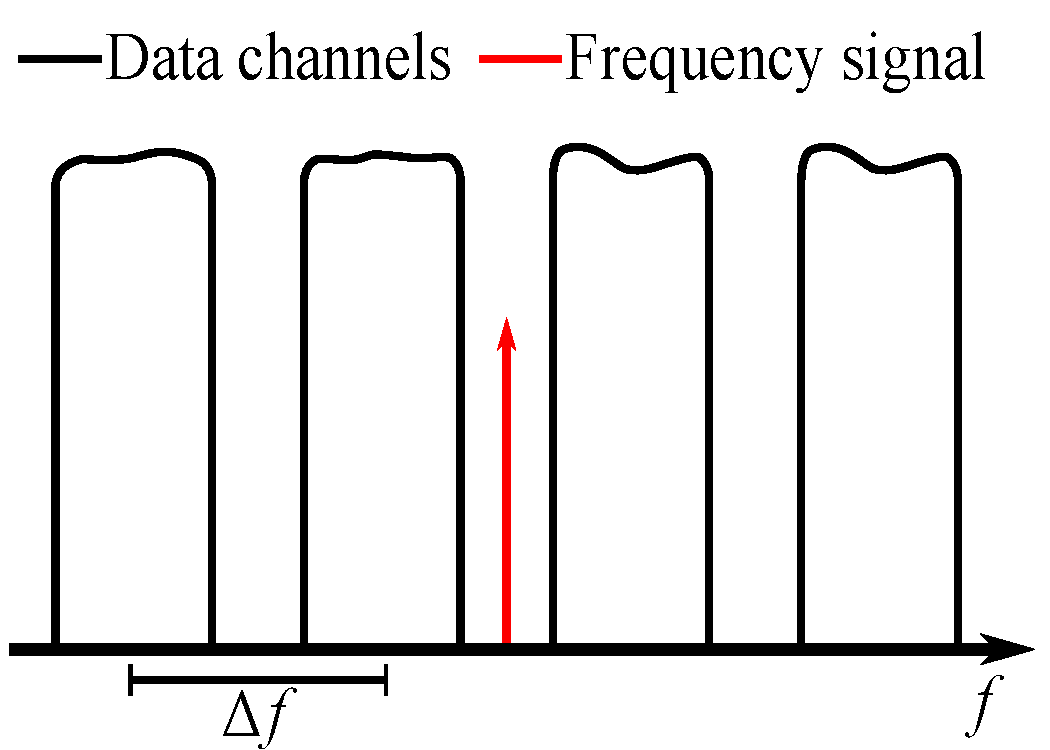
\includegraphics[scale=0.6]{img/system.pdf}
	\renewcommand{\baselinestretch}{1}
	\small\normalsize
	\caption{Desired frequency domain placement of the frequency signal.	\label{fig:system}}
\end{figure}
\renewcommand{\baselinestretch}{2}
\small\normalsize

We will study an optical fiber communication system with multiple WDM data channels centered around the wavelength $1530$ nm and with a bandwidth of $10$ GHz for each channel. The data signals are modulated as non-return-to-zero on-off-keyed (NRZ-OOK) symbols. The optical fiber is a single-mode fiber in which light propagation is impaired by second-order dispersion, the Kerr nonlinearity, and attenuation \cite{agrawal2012fiber,Agrawal2013}. Brillouin scattering, Raman scattering, and Rayleigh scattering can also impair light propagation \cite{Boyd2003}.

In this chapter, we first examine coupled propagation equations for a single data channel and a frequency signal that are separated in the frequency domain. Then, we generalize the coupled equations to account for multiple data channels and a single frequency signal. We further examine each of the impairment terms in the equations, and we will give suitable conditions under which they can be neglected when calculating the phase stability. We will then show that the impairment due to cross-phase modulation is the primary optical source of phase instability.

\section{Coupled Propagation Equations} \label{sec:cnlse}

We begin by considering the interaction of a single data channel and a frequency signal and derive their propagation equations. The small bandwidth of an optical signal compared to the central frequency in an optical fiber allows us to use a slowly varying envelope approximation for the propagation of light \cite{Agrawal2013}. If we consider the interaction of a frequency signal with a single data channel, the electric field becomes a sum of the products of a rapidly varying carrier signal and a slowly varying envelope,
%
\begin{equation}
\mathbf{E}(\mathbf{r}, t) = \frac{1}{2}\hat{\mathbf{x}}\left[ E_d\exp(-i\omega_dt) + E_f\exp(-i\omega_ft)\right] + c.c.,
\end{equation}
%
where $\hat{\mathbf{x}}$ is the direction of polarization, $\omega_j$ for $j=d,f$ are the carrier frequencies for a data channel and the frequency signal respectively, and the $E_j$ are the slowly varying time envelopes. We assume that each of the envelopes may be written as
%
\begin{equation}
E_j(\mathbf{r}, t) = F_j(x,y)u_j(z,t)\exp(i\beta_{0j}z),
\end{equation}
%
where $j=d,f$ corresponds to the appropriate envelope, $F_j(x,y)$ is the distribution of the fiber mode in the plane normal to the propagation direction, $u_j(z,t,)$ is the slowly varying amplitude, and $\beta_{0j}$ is the phase shift associated with propagation distance. Separating the propagation and transverse directions is justified by the large discrepancy in the length scales between the transverse and propagation directions \cite{Agrawal2013}. We then obtain an equation for each envelope $u_j$ in the form of coupled nonlinear Schr{\"o}dinger (NLS) equations \cite{Agrawal2013},
%
\begin{equation}
\frac{\partial u_j}{\partial z} + \beta_{1j}\frac{\partial u_j}{\partial t} + \frac{i\beta_{2j}}{2}\frac{\partial^2 u_j}{\partial t^2} + \frac{\alpha_j}{2}u_j = \frac{in_2\omega_j}{c}\left(f_{jj}|u_j|^2 + 2f_{jk}|u_k|^2\right)u_j,
\end{equation}
%
where $j\neq k$, $j,k = d,f$ for the two envelopes, $\beta_{1j} = 1/v_{gj}$ is the corresponding inverse group velocity, $\beta_{2j}$ is the corresponding group velocity dispersion, and $\alpha_j$ is the attenuation. The terms on the right-hand side represent the nonlinear impairment, $n_2$ is the nonlinear Kerr parameter, and the $f_{jk}$ are the overlap integrals defined as
%
\begin{equation}
f_{jk} = \frac{\int_{-\infty}^{\infty}\int_{-\infty}^{\infty} |F_j(x,y)|^2|F_k(x,y)|^2dxdy }{\int_{-\infty}^{\infty}\int_{-\infty}^{\infty} |F_j(x,y)|^2dxdy\int_{-\infty}^{\infty}\int_{-\infty}^{\infty}|F_k(x,y)|^2dxdy}.
\end{equation}
%
Since the system that we consider uses conventional single-mode fibers, the overlap integrals $f_{jk}$ are all nearly the same. We neglect the differences and write the integrals as $f_{dd} = f_{df} = f_{ff} = 1/A_{\text{eff}}$. This approximation allows us to simplify the right-hand side further by introducing the nonlinear parameter $\gamma = (n_2\omega_j)/(cA_{\text{eff}})$. Though the $\omega_j$ and $A_{\text{eff}}$ have a frequency dependence, this dependence is weak, and $\gamma$ remains fairly constant around the $1.5$-$\mu$m wavelength range that is used for optical communications \cite{Agrawal2013}.

The two coupled equations become
%
\begin{subequations}
\begin{align}
\frac{\partial u_d}{\partial z} + \beta_{1d}\frac{\partial u_d}{\partial t} + \frac{i\beta_{2}}{2}\frac{\partial^2 u_d}{\partial t^2} + \frac{\alpha}{2}u_d &= i\gamma\left(|u_d|^2 + 2|u_f|^2\right)u_d, \label{eq:cdprop} \\
\frac{\partial u_f}{\partial z} + \beta_{1f}\frac{\partial u_f}{\partial t} + \frac{i\beta_{2}}{2}\frac{\partial^2 u_f}{\partial t^2} + \frac{\alpha}{2}u_f &= i\gamma\left(|u_f|^2 + 2|u_d|^2\right)u_f. \label{eq:cfprop}
\end{align}
\end{subequations}
%
It is useful to transform Eqs. \ref{eq:cdprop} and \ref{eq:cfprop} by using a retarded time. We set $T = t - \beta_{1f}z$ and $z' = z$. Then, we use the chain rule to obtain
%
\begin{subequations}
\begin{align}
\frac{\partial u_j}{\partial z} &= \frac{\partial u_j}{\partial z'}\frac{\partial z'}{\partial z} + \frac{\partial u_j}{\partial T}\frac{\partial T}{\partial z} =  \frac{\partial u_j}{\partial z'} - \beta_{1f}\frac{\partial u_j}{\partial T}, \\
\frac{\partial u_j}{\partial t} &= \frac{\partial u_j}{\partial z'}\frac{\partial z'}{\partial t} + \frac{\partial u_j}{\partial T}\frac{\partial T}{\partial t} =  \frac{\partial u_j}{\partial T}, \\
\frac{\partial^2 u_j}{\partial t^2} &= \frac{\partial^2 u_j}{\partial T^2}.
\end{align}
\end{subequations}
%
This transformation removes the term proportional to $\beta_{1f}$ in Eq.~\ref{eq:cfprop}, and the corresponding term in Eq.~\ref{eq:cdprop} becomes proportional to $\delta = \beta_{1d} - \beta_{1f} = (v_{gf} - v_{gd})/(v_{gf}v_{gd})$, so that we obtain
%
\begin{subequations}
\begin{align}
\frac{\partial u_d}{\partial z'} + \delta\frac{\partial u_d}{\partial T} + \frac{i\beta_{2}}{2}\frac{\partial^2 u_d}{\partial T^2} + \frac{\alpha}{2}u_d &= i\gamma\left(|u_d|^2 + 2|u_f|^2\right)u_d, \label{eq:dataprop} \\
\frac{\partial u_f}{\partial z'} + \frac{i\beta_{2}}{2}\frac{\partial^2 u_f}{\partial T^2} + \frac{\alpha}{2}u_f &= i\gamma\left(|u_f|^2 + 2|u_d|^2\right)u_f. \label{eq:freqprop}
\end{align}
\end{subequations}
%

The two terms that are dependent on the optical powers of the signals in the propagation equations represent two different nonlinear phenomena---self-phase modulation and cross-phase modulation \cite{Agrawal2013}. Four-wave mixing is a third nonlinear phenomenon due to the Kerr effect \cite{Agrawal2013,Boyd2003}. This phenomenon does not play a role when only two well-separated frequencies are present, except near the zero dispersion point, since it will not be phase-matched. However, four-wave mixing can lead to phase-matched contributions that affect the signal propagation in a system with multiple data channels.

\section{Multiple Data Channels} \label{sec:multiple}

In the previous section, we showed how two co-propagating signals can nonlinearly couple, creating parasitic signals and inducing a phase shift on each other. Multiple data channels will also couple with the frequency signal and each other. Hence, every data channel in the system can contribute a phase shift to the frequency signal. If there are $n$ data channels at center frequencies $\omega_k$, then we obtain $n+1$ propagation equations,
%
\begin{subequations}
\begin{align}
\frac{\partial u_{dk}}{\partial z'} + \delta_k\frac{\partial u_{dk}}{\partial T} + \frac{i\beta_{2}}{2}\frac{\partial^2 u_{dk}}{\partial T^2} + \frac{\alpha}{2}u_{dk} &= i\gamma\left(|u_{dk}|^2 + 2|u_f|^2 + 2\sum_{\substack{m=1\\ m\neq k}}^n|u_{dm}|^2\right)u_{dk}, \label{eq:mdataprop} \\
\frac{\partial u_f}{\partial z'} + \frac{i\beta_{2}}{2}\frac{\partial^2 u_f}{\partial T^2} + \frac{\alpha}{2}u_f &= i\gamma\left(|u_f|^2 + 2\sum_{m=1}^n|u_{dm}|^2\right)u_f. \label{eq:mfreqprop}
\end{align}
\end{subequations}
%
where the subscript $k,m$ in the data envelopes refers to the $k$th or $m$th data channel and the $\delta_k$ refers to the difference $\beta_{1k} - \beta_{1f}$. The parameters $\beta_2$, $\alpha$, and $\gamma$ can be treated as constant over the frequency range of our frequency signal and data channels.

Four-wave mixing now becomes a concern if $\omega_k + \omega_m = 2\omega_f$ and will appear in the frequency signal if they also satisfy the phase-matching condition $\beta(\omega_k) + \beta(\omega_m) = 2\beta(\omega_f)$. If those two conditions are satisfied, then Eq.~\ref{eq:mfreqprop} must be modified to include the four-wave mixing term, $2\gamma u_f^*u_mu_n$. These two conditions are only simultaneously satisfied when the frequency signal is close to the zero-dispersion wavelength \cite{Agrawal2013}.

We are now prepared to summarize the optical impairments found in the propagation equations \ref{eq:mdataprop} and \ref{eq:mfreqprop}. These impairments appear in commercial optical fiber communication systems and must be limited or compensated to achieve reliable high-data-rate communications. In contrast to data channels, frequency signals do not require a large bandwidth. However, they are intrinsically analog signals that do require high accuracy. Hence, the strategies to calculate the effect of optical impairments and limit their impact are different than is the case for data channels.

\section{Scattering} \label{sec:scattering}

The previous sections outline a propagation medium with negligible defects and no vibrations. The optical fiber has density fluctuations created by manufacturing, electrostriction, or optical absorption. These fluctuations cause light scattering, referred to as Rayleigh scattering \cite{Boyd2003}. Light can also interact with vibrations in the crystal lattice of the optical fiber and cause scattering referred to as Raman and Brillouin scattering \cite{Boyd2003}. The amount of scattering increases with the presence of more photons; so, limiting the optical power of the frequency signal will limit the scattering noise.

Experiments have shown that Rayleigh scattering can be significantly reduced by modulating the input signal \cite{Okusaga:13}. The appropriate modulation is a frequency modulation of the frequency signal
%
\begin{equation}
	\label{eq:modulation}
	\omega_{\text{mod}} = \Delta\omega\sin(\omega_mt + \phi_m),
\end{equation}
%
where $\omega_m$ is the modulation frequency, $\Delta\omega$ is the modulation depth, and $\phi_m$ is the phase difference between the modulation and light fields\cite{menyukIFCS2015}. A modulation frequency between $1$ kHz and $10$ kHz with a large modulation depth of $10$ MHz is optimal \cite{menyukIFCS2015}. Hence, the frequency signal should have a bandwidth of about $10$ MHz.

We give further details on scattering limitations later in Sec. \ref{sec:impair}.

\section{Optical Impairments} \label{sec:impair}

In the previous sections, we showed how the Kerr effect leads to multiple nonlinear terms. In this section, we describe how each of the terms relates to an optical impairment and how that impairment affects the frequency signal. In our analysis, we discuss conditions under which many of the optical impairments become negligible.

\subsection{Attenuation and Amplified Spontaneous Emission (ASE) Noise}
%
Attenuation appears in Eq. \ref{eq:mfreqprop} as
%
\begin{equation}
\diffp{u_f}{z} = -\frac{\alpha}{2}u_f.
\end{equation}
%
The attenuation is due to absorption and Rayleigh scattering and will lead to an exponential decrease of the optical power \cite{agrawal2012fiber}. Amplifiers are spaced periodically to compensate for the loss of optical power, but they add amplified spontaneous emission (ASE) noise. ASE noise is accurately described over the bandwidth of an optical signal as a white noise source with noise power \cite{agrawal2012fiber}
%
\begin{equation}
\sigma^2_{\text{ASE}} = n_{\text{sp}}h\nu_0 (G-1)\Delta\nu,
\end{equation}
%
where $n_{\text{sp}}$ is called the spontaneous emission factor, $h$ is Planck's constant, $\nu_0$ is the center frequency, $G$ is the gain of the amplifier, and $\Delta\nu$ is the bandwidth of the signal. 

We will consider an optical communication system that has a length of $800$ km and an $80$-km amplifier separation, operating at the wavelength $1.5$ $\mu$m with loss $\alpha_{\text{dB}} = 0.2$ dB/km. There are a total of $10$ amplifiers, each of which has a gain $G=40$. We will assume that each amplifier has a noise figure $n_{\text{sp}} = 2$, which is a typical value \cite{agrawal2012fiber}. If we suppose that the bandwidth of the frequency signal is $10$ MHz, then the total noise power is $1$ nW. If the frequency signal has a power of $1$ $\mu$W or above, the effect of the noise on the frequency signal will be negligible, while its power is small compared to the power in a data signal, which is typically on the order of $1$ mW after each amplifier.

\subsection{Chromatic Dispersion}

The dispersion appears in Eq.~\ref{eq:mfreqprop} as
%
\begin{equation}
\diffp{u_f}{z} = -\frac{i\beta_{2}}{2}\diffp{^2u_f}{T^2}.
\end{equation}
%
This impairment leads to pulse spreading of the optical signal because its frequency components travel at different velocities. The time spread due to dispersion is \cite{agrawal2012fiber}
%
\begin{equation}
\tau_{\text{disp}} = -\frac{2\pi c}{\lambda^2}\beta_{2f} L\Delta \lambda,
\end{equation}
%
where $L$ is the length of the fiber, and $\Delta\lambda$ is the range of wavelengths. For the optical communication system in the previous example and a frequency signal centered at a wavelength $\lambda = 1.5$ $\mu$m, we find $\tau_{\text{disp}} = 1$ ps. By contrast, the time slot of a single bit at $10$ Gbps occupies $100$ ps; so, dispersion can be neglected for the frequency signal. In this respect, the frequency signal differs significantly from a data signal, which typically has a bandwidth on the order of $10$ GHz.


\subsection{Self-Phase Modulation (SPM)}

The term
\begin{equation}
\diffp{u_f}{z} = i\gamma|u_f|^2u_f
\end{equation}
in Eq.~\ref{eq:mfreqprop} corresponds to self-phase modulation. This effect leads to a phase shift that is proportional to the signal power. Thus, linear attenuation limits the effect over some length after each amplifier. The effective length is $L_{\text{eff}} = (1/\alpha)[1-\exp(-\alpha L)]$, so that $L_{\text{eff}} \approx 20$ km for $\alpha_{\text{dB}} = 0.2$ dB/km \cite{Agrawal2013}. The maximum phase shift due to self-phase modulation between two amplifiers is \cite{Agrawal2013}
%
\begin{equation} \label{eq:maxspm}
\phi_{\text{SPM}} = \gamma P_f L_{\text{eff}},
\end{equation}
%
where $P_f$ is the average power of the frequency signal after an amplifier. The total maximum phase shift is given by Eq.~\ref{eq:maxspm} multiplied by the number of amplifiers in the fiber link. For our system, we have $\gamma = 1.3$ W$^{-1}$km$^{-1}$ and $L_{\text{eff}} = 20$ km with $10$ amplifiers. If we impose an upper bound on $\phi_{\text{SPM}}$ of $1$ radian, then the upper bound on the frequency signal power is $3.8$ mW.

\subsection{Four-Wave Mixing (FWM)}

The term
%
\begin{equation}
i\gamma u_f^*u_{dm}u_{dn}
\end{equation}
%
corresponds to four-wave mixing. For any two data signals centered at $\omega_m$ and $\omega_n$ with corresponding wavenumbers $\beta(\omega_m)$ and $\beta(\omega_n)$, four-wave mixing (FWM) creates a parasitic wave whenever $\omega_m + \omega_n = 2\omega_f$ and $\beta(\omega_m) + \beta(\omega_n) = 2\beta(\omega_f)$. This phase-matching condition is avoidable as long as the signals are located away from the zero-dispersion wavelength of the fiber. Frequency sources have a central wavelength that slightly wanders and a narrow bandwidth. Therefore, placing the frequency signal greater than five times its bandwidth away from the zero-dispersion wavelength prevents any portion of the spectrum of the frequency signal from phase-matching and will eliminate this impairment \cite{menyukIFCS2015}. We write this requirement as $\lambda-\lambda_0 > 5 \Delta\lambda$, where $\lambda$ is the central wavelength of the frequency signal signal, $\lambda_0$ is the zero-dispersion wavelength, and $\Delta\lambda$ is the bandwidth of the frequency signal.

\subsection{Rayleigh Scattering}

An optical fiber has random density fluctuations that are created during the fiber's fabrication. These fluctuations are the primary source of attenuation in the fiber, on the order of $0.12$--$0.17$ dB/km at $1.5$ $\mu$m \cite{agrawal2012fiber}. Additionally, Rayleigh scattering adds noise to a narrowband frequency signal; however, this noise can be suppressed by a frequency modulation with a bandwidth that is greater than about $10$ MHz \cite{Okusaga:13}.

\subsection{Brillouin and Raman Scattering}

Brillouin and Raman scattering are due to light coupling with vibrations in the crystal lattice of the optical fiber and convert the light to lower frequencies. Brillouin scattering couples with acoustic waves and Raman scattering couples with vibrational waves.

Brillouin scattering only occurs when a phase matching condition is met, $\omega_{\text{orig}} = \omega_{\text{new}} + \omega_{\text{acoustic}}$ and $\beta_{\text{orig}} = \beta_{\text{new}} + \beta_{\text{acoustic}}$, where $\omega_{\text{orig}}$ and $\beta_{\text{orig}}$ are the frequency and wavenumber of the incident wave, $\omega_{\text{new}}$ and $\beta_{\text{new}}$ are the frequency and wavenumber of the created optical wave, and $\omega_{\text{acoustic}}$ and $\beta_{\text{acoustic}}$ are the frequency and wavenumber for the acoustic wave. The large difference between the velocities of the optical waves and the acoustic wave means that the phase matching condition only occurs when the created wave propagates in the direction opposite to that of the incident wave ($\beta_{\text{new}}$ is negative). A Brillouin scattered wave grows from thermal noise at a rate proportional to the incident light intensity. If the growth rate is greater than the loss due to attenuation, then the created wave grows exponentially. This growth sets a threshold on the incident wave's power \cite{Boyd2003, agrawal2012fiber}
%
\begin{equation}
P_{\text{max,B}} = \frac{21A_{\text{eff}}}{L_{\text{eff}}g_B},
\end{equation}
%
where $L_{\text{eff}}$ is the effective fiber length, $A_{\text{eff}}$ is the fiber effective area, and $g_B$ is the Brillouin gain. Brillouin scattering is a narrowband process with a gain bandwidth on the order of $100$ MHz which our frequency signal can fit within. The actual power threshold will depend on the system and can range between $1$--$10$ mW \cite{agrawal2012fiber}. If we set an upper limit of $1$ mW on the frequency signal, then we avoid the effect of Brillouin scattering.

Raman scattering is similar to Brillouin scattering except that it is a broadband process on the order of $20$ THz \cite{Boyd2003}. In this case, the power threshold is \cite{agrawal2012fiber}
%
\begin{equation}
P_{\text{max,R}} = \frac{16A_{\text{eff}}}{L_{\text{eff}}g_R},
\end{equation}
%
where we use the same parameters as before and $g_R$ is the Raman gain. Raman scattering sets an upper threshold of $500$ mW which is well above the threshold set by other optical impairments.


\subsection{Cross-Phase Modulation (XPM)}

The remaining term,
\begin{equation}
\diffp{u_f}{z} = i2\gamma|u_d|^2u_f,
\end{equation}
corresponds to cross-phase modulation (XPM), which leads to cross-talk between two signals. This effect on the frequency signal becomes negligible when the group velocity difference between the data channel and the frequency signal is large, which occurs when the frequency signal and data channel are spaced at least one data channel separation away. Therefore, the effects of XPM on the frequency signal only has to be computed for the two neighboring data channels. Since our goal is to place the frequency signal between two data channels, XPM is the primary source of frequency distortion. 

The limitation on the optical power of the frequency signal ($\ll 1$ mW) implies that the effect of XPM due to the frequency signal on the data channels will be much less than a radian and can be neglected.

\section{Phase distortion of the frequency signal due to XPM} \label{sec:noisexpm}

Data signals can be modeled as random bit strings. The average behavior of two neighboring data channels on the frequency signal will be equal as long as the frequency signal is placed in the middle of the frequency gap between the data channels. We simplify our analysis of the effect of XPM on the frequency signal by replacing the effect of the two neighboring data signals with a doubling of the effect of a single data signal.

Applying the limits on the system parameters that we have obtained, Eqs. \ref{eq:mdataprop} and \ref{eq:mfreqprop} simplify to the following equations,
%
\begin{subequations}
\begin{align}
\label{eq:simpledfreq}
&\diffp{u_f}{z} = i4\gamma|u_d|^2u_f, \\
\label{eq:simpleddata}
&\diffp{u_d}{z} + \delta\diffp{u_d}{T} + \frac{i\beta_{2}}{2}\diffp{^2u_d}{T^2} + \frac{\alpha}{2}u_d = i\gamma|u_d|^2u_d.
\end{align}
\end{subequations}
%
The dispersion, SPM, FWM, and attenuation are negligible for the frequency signal. The non-neighboring data channels are sufficiently separated in frequency to neglect their contribution to XPM. The effect of XPM has been doubled to represent the mean behavior of the two neighboring data signals. Low optical power of the frequency signal makes the effect of XPM on the data signal negligible. 

The frequency signal has the form $u_f(z,T) = u_f(0,T)\exp[i\phi(z,T)]$, where $u_f(0,T)$ is the initial frequency signal and $\phi(z,T)$ is phase distortion due to XPM. We may integrate Eq.~\ref{eq:simpledfreq}, from which it follows that
%
\begin{equation} \label{eq:phasedistort}
	\phi(z,T) = 4\gamma\int_0^{z} |u_d(\zeta, T)|^2 d\zeta.
\end{equation}
%
The data signal is subject to the effects of loss, dispersion, a time shift due to the group velocity difference from the frequency signal, and self-phase modulation. The phase distortion of the frequency signal depends entirely on the evolution of the data signal as it propagates through the fiber.

\section{Chapter Remarks} \label{sec:3conc}

\renewcommand{\baselinestretch}{1}
\small\normalsize

\begin{table}[h]
	\raggedright
	\begin{tabular}{| c | c | c |}
		\hline
		Impairment & Limits & Threshold \\ \hhline{|=|=|=|}
		Attenuation and ASE & Optical Power & $\ge 1$ nW \\ \hline
		Rayleigh Scattering & Frequency Modulation & $\ge 10$ MHz \\ \hline
		Brillouin Scattering & Optical Power & $< 1$ mW \\ \hline
		Raman Scattering & Optical Power & $< 500$ mW \\ \hline
		Self-Phase Modulation & Optical Power & $< 3.8$ mW \\ \hline
		Four-Wave Mixing & Central Frequency & $\lambda - \lambda_0 > 5\Delta\lambda$ \\ 
		\hline
	\end{tabular}
	\caption{Summary of the limits on the frequency signal imposed by the optical impairments. \label{table:limits}}
\end{table}

\renewcommand{\baselinestretch}{2}
\small\normalsize

Table \ref{table:limits} summarizes the various limits we place on the frequency signal to reduce the effect of optical impairments. By limiting the frequency signal's optical power and its bandwidth, we can limit the causes of phase distortion due to optical impairments. As a consequence, the distortion will be dominantly due to XPM. In the next chapter, we perform computations to estimate $\phi(z,T)$ using typical system parameters for a commercial optical fiber communication system.


	\chapter{Results}
\label{chap:results}

\section{Introduction}

In the previous chapter, we described the parameters of a commercial WDM optical fiber communication system with a frequency signal that is located between two data channels, as shown in Fig.~\ref{fig:system}. Given reasonable system parameters, we showed that the dominant optical impairment is XPM, given by Eq.~\ref{eq:phasedistort}, and all other optical impairments can be made negligible.

It follows that the phase distortion depends on the length of fiber, the frequency separation between the frequency signal and the data channels, and the power of the neighboring data channels as they change over the course of their propagation. We will now vary these parameters and investigate their effect on the stability of the frequency signal.

We choose a value for the data channel power that is typical in commercial optical communication systems. These values are chosen to minimize nonlinear distortion in the data signals \cite{Agrawal2013, agrawal2012fiber}. Hence, we neglect the nonlinear distortion of the data signals when calculating $\phi(z,t)$ and focus on the effect of dispersion. The evolution of the data signal is then easily obtained in the Fourier domain, and we find
%
\begin{equation} \label{eq:datasol}
u_d(z,T) = \frac{1}{2\pi} \int_{-\infty}^{\infty} U_d(0, \omega')\exp\left(-\frac{\alpha}{2} z + i\delta\omega' z + \frac{i}{2}\beta_2\omega'^2z-i\omega' T\right) d\omega' ,
\end{equation}
%
where $U_d(0,\omega)$ is the Fourier spectrum of the data signal at $z=0$, defined as
\begin{equation}
U_d(0,\omega) = \int_{-\infty}^{\infty} u_d(0, t')\exp(i\omega t')dt'.
\end{equation}

We begin by investigating the distribution of the power of the data signal $|u_d|^2$ as a function of length $z$. The on-off-keyed, nonreturn-to-zero (OOK-NRZ) symbols of the data signal change over the length of the fiber due to dispersion, self-phase modulation, and attenuation. We first study a system in which attenuation is neglected. We then add the effect of attenuation. Finally, we study the system behavior as the group velocity difference due to the frequency separation between the neighboring data channels and frequency signal increases.

\section{Simulation Parameters}

The simulated data signal is a $2^{10}-1$ pseudorandom binary sequence (PRBS) \cite{PRBS} that is OOK-NRZ modulated with optical power of $1$ mW with periodic boundary conditions. A PRBS has properties that resemble a random sequence. It is approximately delta-correlated, and has an almost equal number of $0$s and $1$s. As a consequence, the statistical properties of the signal converges more rapidly as the sequence length increases than if the string of $0$s and $1$s are randomly chosen. PRBS signals are commonly used in both computer simulations and laboratory experiments to model data channels. The length of the string is chosen so that the string does not repeat as the data channel travels through a fixed time point in the frequency signal.

The fiber has an attenuation of $\alpha = 0.2$ dB/km, group velocity dispersion $\beta_2 = -22$ ps$^2$/km, and Kerr nonlinearity $\gamma = 1.3$ W$^{-1}$km$^{-1}$. The data signal has a central wavelength of $1530$ nm with inverse group velocity difference $\delta = 1$ ps/km relative to the frequency signal. These parameters are typical for optical fiber communication systems \cite{agrawal2012fiber,Agrawal2013}. We will vary some of these parameters in the following sections as we study the changes in the XPM-induced phase distortion.


\section{Without Attenuation}

We first neglect attenuation in order to provide a baseline against which to determine its effect.

During propagation, the optical power in each bit of the data signal spreads outside of its time slot into the time slots of its neighbors. After some long distance, the expected power in each time slot will become the same. Therefore, the variance of the data signal's optical power is expected to decrease as a function of fiber length, although there will be statistical fluctuations in the pseudo-random signal that we are using. Figure~\ref{fig:NACalcVar} shows the data signal power variance as the distance varies up to $800$ km. Since there is no attenuation, the mean of the data signal power is constant. Though not shown in the figure, longer propagation distances yield a variance on the order of $1.8 \times 10^{-7}$ W$^2$.
%
\begin{figure}[htb]
	\raggedright
	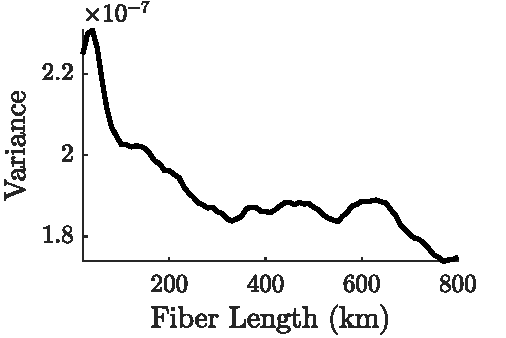
\includegraphics[scale=0.8]{img/NACalcVar}
	\renewcommand{\baselinestretch}{1}
	\small\normalsize
	\caption{Data channel optical power variance vs. fiber length.} \label{fig:NACalcVar}
\end{figure}
\renewcommand{\baselinestretch}{2}
\small\normalsize

The phase shift $\phi$ grows as a function of distance because the frequency signal experiences cross-talk from the data signal, which accumulates over the propagation length. Figures \ref{fig:NAPhiMean}a and \ref{fig:NAPhiVar}b show the mean and variance of the phase shift of the frequency signal due to XPM. The mean of $\phi$ grows linearly with respect to the fiber length because without attenuation the average energy in the data signal is constant. As a consequence, the mean additive phase error can be compensated.
%
\begin{figure}[htb]
	\raggedright
	\begin{tabular}{c c}
		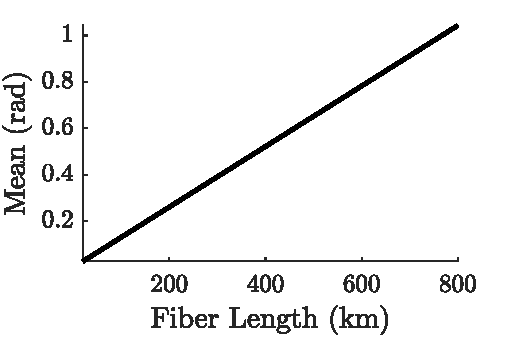
\includegraphics[width=0.5\linewidth]{img/NAPhiMean} & 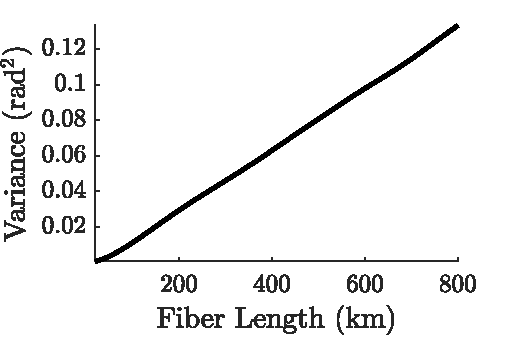
\includegraphics[width=0.5\linewidth]{img/NAPhiVar} \\
		(a) & (b)
	\end{tabular}
	\renewcommand{\baselinestretch}{1}
	\small\normalsize
	\caption{(a)\label{fig:NAPhiMean} Mean of $\phi$ vs. fiber length (b)\label{fig:NAPhiVar} Variance of $\phi$ vs. fiber length.}
\end{figure}
\renewcommand{\baselinestretch}{2}
\small\normalsize

We now quantify the phase deviation using the measures that we introduced in Chapter \ref{chap:time_stability}. We first consider the first structure equation, $D^{(1)}_\phi = \langle [\phi(t+\tau) - \phi(t)]^2 \rangle$, which represents the mean phase accumulation. As we discussed in Chapter \ref{chap:time_stability}, the structure functions are related to the autocorrelation function. A typical data signal is a collection of apparently random bits that are uncorrelated with each other. As the data signal propagates through the fiber, the optical energy associated with each bit occupies a larger amount of time due to dispersion, so that the amount of time in which a bit is correlated with itself increases. Figure \ref{fig:NAPhaseStability} shows $\left[D^{(1)}_\phi\right]^{1/2}$ at different lengths. The phase deviation becomes constant after a short amount of time.

Figure \ref{fig:NAAllanDev} shows the Allan deviation. After averaging the fractional frequency over a time interval on the order of the duration of the bit pulse, $\tau = 10^{-10}$ s, the Allan deviation starts to fall off at a rate proportional to $\tau^{-1}$. This falloff signifies that rapidly oscillating errors are being averaged out. We expect the falloff to continue indefinitely because XPM contributes no long-term frequency drift. We have computed the Allan deviation up to $10$ ns, at which point the trend proportional to $\tau^{-1}$ is apparent. Extrapolating the $\tau^{-1}$ dependence to longer averaging times, we find that the Allan deviation is $3\times 10^{-15}$ at $\tau = 1$ s, and $3\times 10^{-18}$ at $\tau=10^3$ s.

%
\begin{figure}[htb]
	\raggedright
	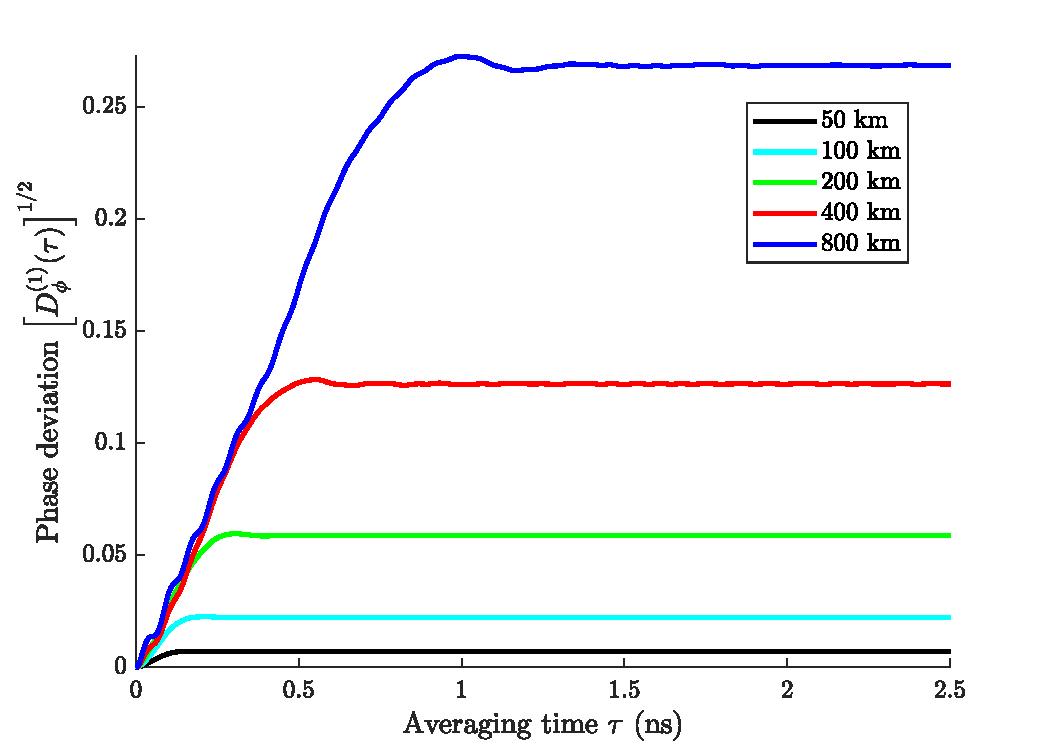
\includegraphics[scale=0.8]{img/NAPhaseStability}
	\renewcommand{\baselinestretch}{1}
	\small\normalsize
	\caption{Phase deviation without attenuation.} \label{fig:NAPhaseStability}
\end{figure}
\renewcommand{\baselinestretch}{2}
\small\normalsize

%
\begin{figure}[htb]
	\raggedright
	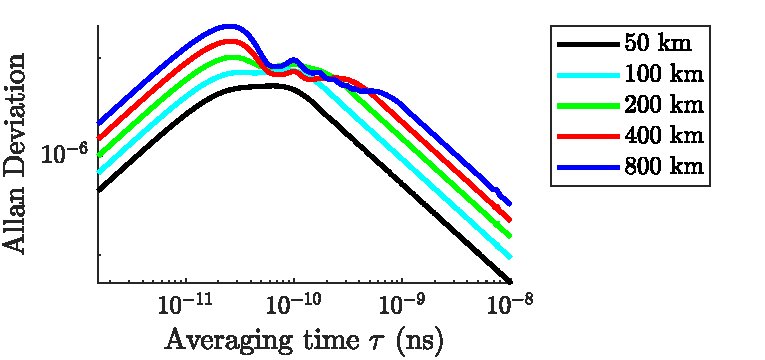
\includegraphics[scale=0.8]{img/NAAllanDev}
	\renewcommand{\baselinestretch}{1}
	\small\normalsize
	\caption{Allan deviation without attenuation.} \label{fig:NAAllanDev}
\end{figure}
\renewcommand{\baselinestretch}{2}
\small\normalsize

\clearpage

\section{Effect of Attenuation}

We now include the effect of attenuation. We expect the phase and frequency instability to be lower than was the case without attenuation because the effective length before the nonlinearity and hence XPM become negligible is $20$ km after each amplifier.

%
\begin{figure}[htb]
	\raggedright
	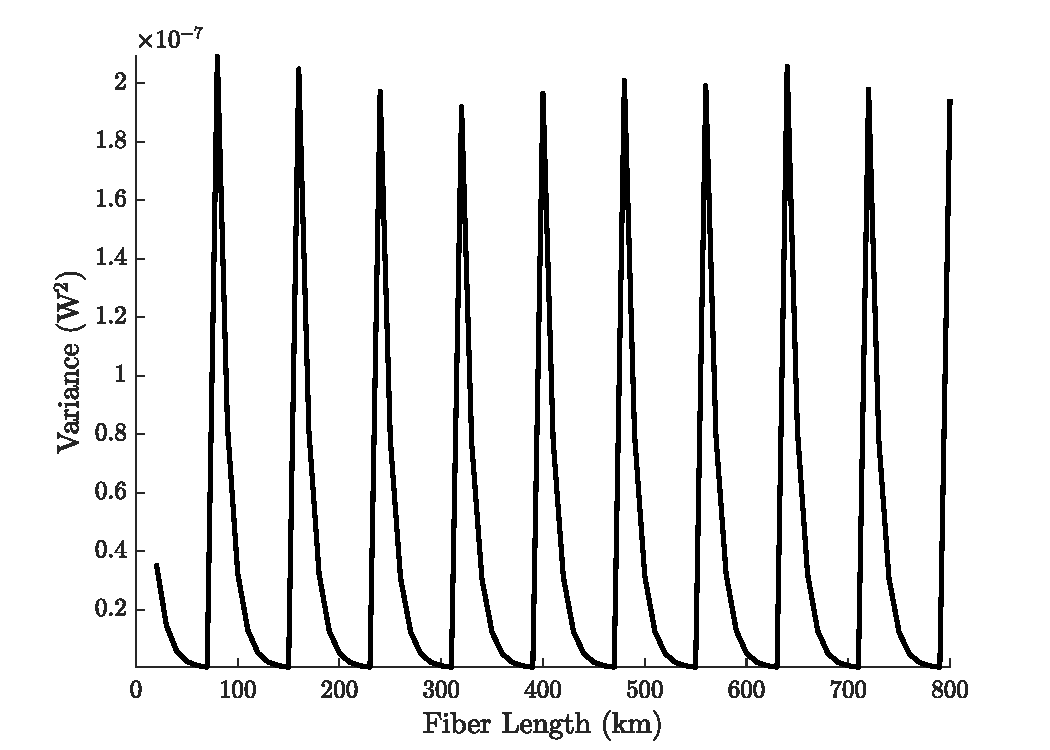
\includegraphics[scale=0.8]{img/ACalcVar}
	\renewcommand{\baselinestretch}{1}
	\small\normalsize
	\caption{Data channel optical power variance vs. fiber length.} \label{fig:ACalcVar}
\end{figure}
\renewcommand{\baselinestretch}{2}
\small\normalsize

First, we compare the variance of the attenuated data signal with the variance without attenuation. Figure~\ref{fig:ACalcVar} shows the data signal's optical power variance. Spikes occur every $80$ km, corresponding to the locations of the amplifiers.

%
\begin{figure}[htb]
	\raggedright
	\begin{tabular}{c c}
		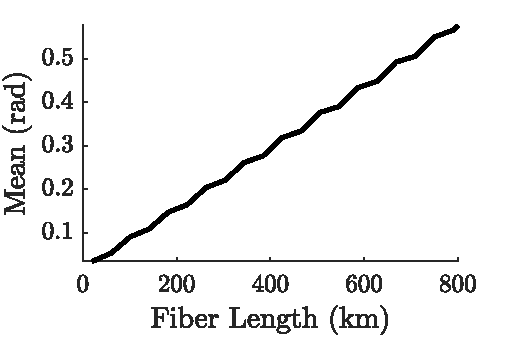
\includegraphics[width=0.5\linewidth]{img/APhiMean} & 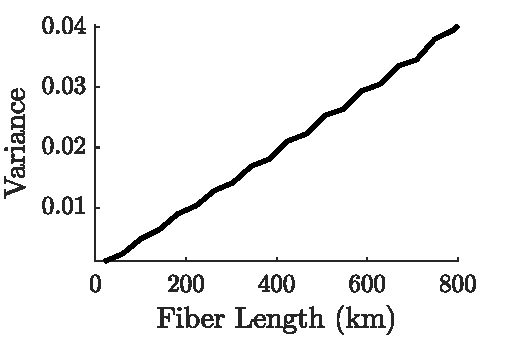
\includegraphics[width=0.5\linewidth]{img/APhiVar} \\
		(a) & (b)
	\end{tabular}
	\renewcommand{\baselinestretch}{1}
	\small\normalsize
	\caption{(a)\label{fig:APhiMean} Mean of $\phi$ vs. fiber length (b)\label{fig:APhiVar} Variance of $\phi$ vs. fiber length.}
\end{figure}
\renewcommand{\baselinestretch}{2}
\small\normalsize

The mean and variance of $\phi$ must also grow over the length of the fiber, but they no longer grow almost linearly because the data signal power varies. Instead, the mean and the variance grow in steps. Figures \ref{fig:APhiMean}a and \ref{fig:APhiVar}b show the mean and variance of $\phi$ respectively, in which flat regions where the data signal power is low are visible. The mean and variance are less than when attenuation was neglected because the average power of the data channels is lower.

%
\begin{figure}[htb]
	\raggedright
	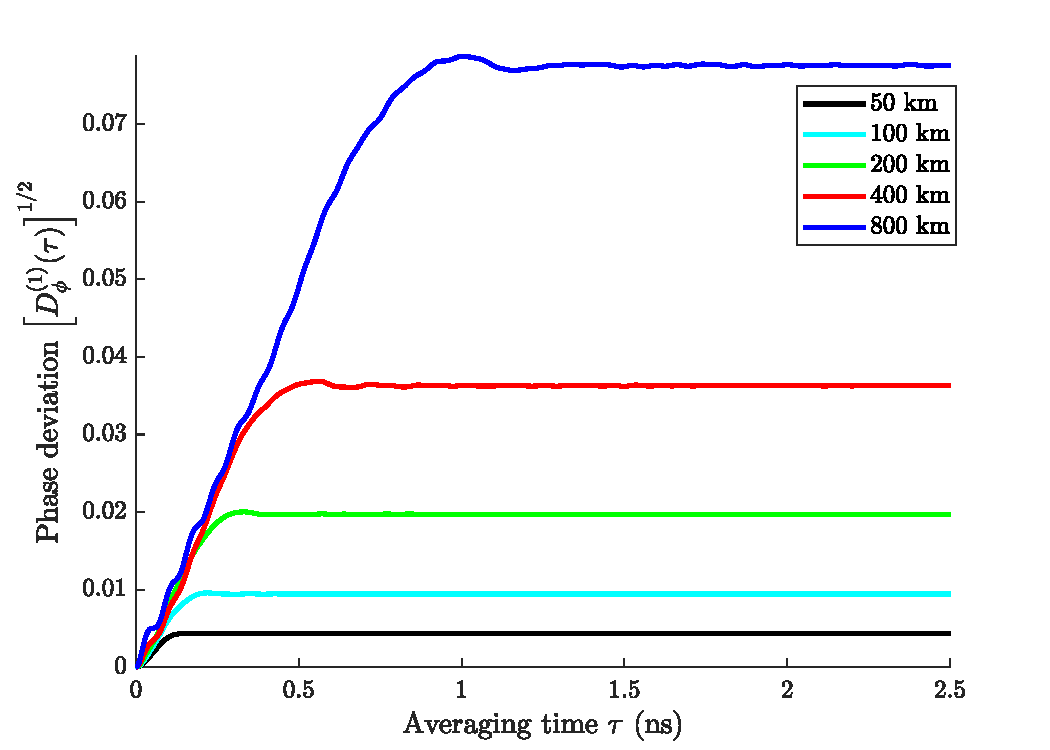
\includegraphics[scale=0.8]{img/APhaseStability}
	\renewcommand{\baselinestretch}{1}
	\small\normalsize
	\caption{Phase deviation with attenuation.} \label{fig:APhaseStability}
\end{figure}
\renewcommand{\baselinestretch}{2}
\small\normalsize%

The phase deviation $\left[D^{(1)}_\phi\right]^{1/2}$ reaches an asymptotic value as was the case when attenuation is neglected. Since the asymptotic value depends on the pulse spreading due to dispersion, the asymptotes occur at the same times. However, the phase deviation will be lower than was the case without attenuation, because the effect of XPM on the frequency signal from the data channels depends on the optical power of the data channels. Figure~\ref{fig:APhaseStability} shows $\left[D^{(1)}_\phi\right]^{1/2}$ for different fiber lengths.

Finally, the Allan deviation will be comparable to the results in the previous section. Figure~\ref{fig:AAllanDev} shows the Allan deviation for several fiber lengths, and we see a similar trend to what we saw without attenuation. At very low averaging times, $\tau < 10^{-11}$ s, there is higher uncertainty than in Figure~\ref{fig:NAAllanDev} due to high frequency ASE noise in the data signal. The Allan deviation will also decrease at a rate proportional to $\tau^{-1}$ after an averaging time interval approximately equal to the bit duration. We perform the same extrapolation as in the previous section, and we find an Allan deviation of $10^{-15}$ at $\tau=1$ s, and $10^{-18}$ at $\tau=10^3$ s.

\clearpage

%
\begin{figure}[htb]
	\raggedright
	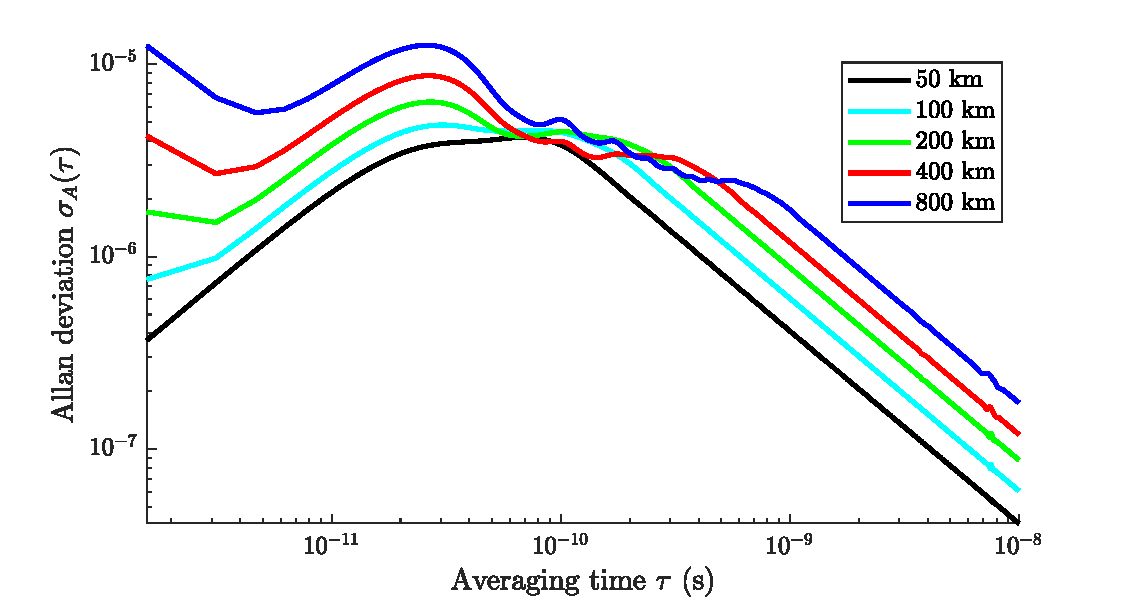
\includegraphics[scale=0.8]{img/AAllanDev}
	\renewcommand{\baselinestretch}{1}
	\small\normalsize
	\caption{Allan deviation with attenuation.} \label{fig:AAllanDev}
\end{figure}
\renewcommand{\baselinestretch}{2}
\small\normalsize%


\section{Varying the Frequency Separation}

The frequency separation between the data channels and the frequency signal will lead to a group velocity difference between the data channels and the signal channels, due to chromatic dispersion. The relative group velocity difference governs the rate at which the data signal travels through a fixed time point in the frequency signal. The group velocity difference is related to the separation between the center frequencies of the data channels and the frequency signal. The value $\delta = (v_{f}-v_{d})/(v_fv_d) = 1$ ps/km is chosen because it corresponds to placing the frequency signal at the midpoint between two neighboring data channels separated by $12.5$ GHz. As the separation between the center frequencies decreases, the group velocity difference decreases and thus $\delta$ decreases. 

Figure~\ref{fig:GVPhaseStability} shows the phase deviation for different frequency spacings between the data and frequency signal. The frequency separation in the figure refers to the separation between the center frequencies of the data channel and the frequency signal. The $6.25$ GHz separation refers to the system described in this thesis, where the frequency signal is placed in the boundaries of two closest neighboring data signals that conform with the ITU grid standard \cite{ITU-T2012}. The $12.5$ GHz separation corresponds to replacing a data channel with the frequency signal. Further separations are used to demonstrate the effect of XPM diminishing as the data channel is placed further away from the frequency signal.

\begin{figure}[htb]
	\raggedright
	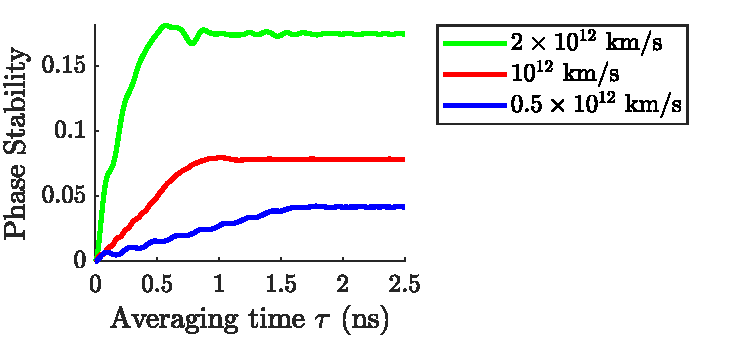
\includegraphics[scale=0.8]{img/GVPhaseStability}
	\renewcommand{\baselinestretch}{1}
	\small\normalsize
	\begin{quote}
		\caption{Phase deviation vs. group velocity difference.} \label{fig:GVPhaseStability}
	\end{quote}
\end{figure}
\renewcommand{\baselinestretch}{2}
\small\normalsize

\section{Comparison to Frequency Transfer Experiments}

Experiments in optical frequency transfer are typically performed on dark fibers or use frequencies alloted to a data channel. Experiments with simple unidirectional fiber optic links have an Allan deviation of $10^{-14}$ with one day of averaging \cite{UniExperiment1, UniExperiment2, UniExperiment3}. Improvements in frequency transfer have reduced the Allan deviation so that it is on the order of $10^{-17}$ with an averaging time of $10^5$ sec \cite{UniExperiment2,Experiment1}. Now, the primary source of phase noise in frequency transfer experiments is random temperature fluctuations over the length of the fiber \cite{TempExperiments}. 

Frequently these experiments are performed on optical fiber links that are in the range of $80$ -- $500$ km. The difference between the lengths of these experiments and our simulation is not a major concern, because the phase noise due to XPM increases as the length of the fiber link increases. We expect the larger distance in our simulations will exaggerate the phase noise due to XPM. Comparing the experiments to our results in the previous sections, we find that the phase noise due to XPM from placing the frequency signal in the interstices of two neighboring data channels is on the order of environmental effects.

\section{Chapter Remarks}

Since the bits in any data signal are uncorrelated, the phase deviation will asymptote after an averaging time that corresponds approximately to the time that it takes a single bit to slide through a constant phase point in the frequency signal. When the relative group velocity is greater, the phase deviation reaches its final value at a smaller distance because the data signal passes through a fixed time point in the frequency signal at a faster rate. 

The Allan deviation represents the expected frequency error. Experiments performing frequency transfer with a frequency signal that occupies an entire data channel on the ITU grid have Allan deviations that are comparable to our simulated values \cite{Serrano2013,cantin2017progress}. In this case, the frequency signal and data channels are separated by many GHz. The source of error in the experiments is environmental fluctuations. We have found that placing a frequency signal in the interstices of two data signals gives a frequency error on the order of environmental effects and should therefore be feasible. Hence, it is not necessary to use an entire data channel to transfer a frequency signal.
	\chapter{Conclusion}

A frequency signal in an optical fiber suffers optical impairments due to the medium. By placing requirements on the location and optical power of the frequency signal, we can eliminate a majority of the impairments.

Systems performing frequency transfer over optical fiber place the frequency signal at a center frequency designated for a data channel which wastes a significant amount of bandwidth. We can solve this issue by moving the frequency signal into the interstices of the data channels. However, placing the frequency signal closer to the data channels will increase the amount of cross-talk which causes an increased amount of phase and frequency error.

We computed the amount of frequency error due to cross-talk using the Allan Deviation and found that it was comparable to environmental effects in experimental setups. This means it is feasible to move the frequency signal to the interstices of two data channels without significant error due to cross-phase modulation.

\section{Future Work}

The length of the optical fiber was chosen to eliminate the effects of self-phase modulation on the data channel. Increasing the length of the transmission to $3000$--$4000$ km, comparable to the length of research institutions in the United States, requires computing the effects of the self-phase modulation. This was avoided in our work because the amount of time necessary to solve the Nonlinear Schr{\"o}dinger Equation using the split-step Fourier method was prohibitively long.
	
	\renewcommand{\baselinestretch}{1}
	\small\normalsize
	\newpage
	\bibliographystyle{ieeetr}
	\bibliography{document}
\end{document}